The main problem with the two previous tests and how we are using the learning algorithm, is that we only have one linear system for each run of the algorithm. A consequences of this is that the algorithm does not learn a preconditioner that could work for some general matrix, but a good preconditioner for that specific matrix, which is what this project is about. A parallel to this is that with only one matrix the algorithm is unnecessary, as we are learning to solve the system with fewer iteration by solving system itself. The only way to solve this is to get more matrices and to have a set matrices for the training part and set to evaluate the learned preconditioner, as to ensure the algorithm is not overfitting to the training data. To do this we will use the 2-dimensional discrete laplace operator, \(\Delta\), with periodic boundary conditions. As the laplace operator has a direct connection to the Dirac operator \(D^2=\Delta\). 

\noindent The \(D\)-dimensional discrete laplace operator can be constructed as such \cite{boutot2026},

\begin{equation}
    \Delta =\sum_{d=1}^{D}\left(\left(\bigotimes_{k=d}^{d-1} I^{(N_k)} \right)\otimes \Delta_{h_d}^{(N_d)} \otimes \left(\bigotimes_{k=d+1}^{D}I^{(N_k)}\right)\right).
\end{equation}
Where \(\Delta_{h_d}^{(N_d)}\) is the \(N_d\times N_d\) 1-dimensional discrete laplace operator, where we have chosen with periodic boundary conditions, for the \(d\)'th dimension is defined as
\begin{equation}
    \Delta_{h_d}^{(N_d)}=\frac{1}{h_d}
    \begin{bmatrix}
    -2 &1 & 0 &\cdots & 0 & 1\\
    1 & -2 &1 & \cdots & 0 & 0\\
    \vdots&\vdots & \ddots & \vdots & \vdots\\
    0 & 0 &0 & \cdots & -2 & 1\\
    1 & 0 &0 & \cdots & 1 & -2
    \end{bmatrix},
\end{equation}
with discretization step size of \(h_d\) and \(N_d\) grid points. \(I^{(N_d)}\) is a \(N_d\times N_d\) identity matrix. \(A\otimes B\) is the Kronecker product defined between two matrices \(A\) and \(B\) of size \(n\times m\) and \(i\times j\) respectively as

\begin{equation*}
    A\otimes B =
    \begin{bmatrix}
    a_{11} B & \cdots & a_{1m}B\\
    \vdots  & \ddots & \vdots\\
    a_{n1}B & \cdots & a_{nm}B
    \end{bmatrix},
\end{equation*}
and the resulting matrix is of size \(n\cdot i \times m\cdot j\).

\noindent The 2-dimensional laplace can then be written as

\begin{equation}\label{eq: 2d laplace Kronecker}
    \Delta_{h_1}^{(N_1)}\otimes I^{(N_2)} + I^{(N_1)}\otimes \Delta_{h_2}^{(N_2)}.
\end{equation}

Because we want the matrices to be invertible, the matrix has to be square and the Kronecker produces a matrix of size \(n\cdot i \times m \cdot j\), we will use the same discretization for both dimensions, \(N_1=N_2=N\) and for simplicity both of the discretization step sizes will be set to one, \(h_1=h_2=1\). An example with \(N=6\) the 2-dimension discrete laplace operator can be seen in figure \ref{fig: 2d laplace heat map} as a heatmap, with zeros removed for clarity .

\begin{figure}[H]
    \center
    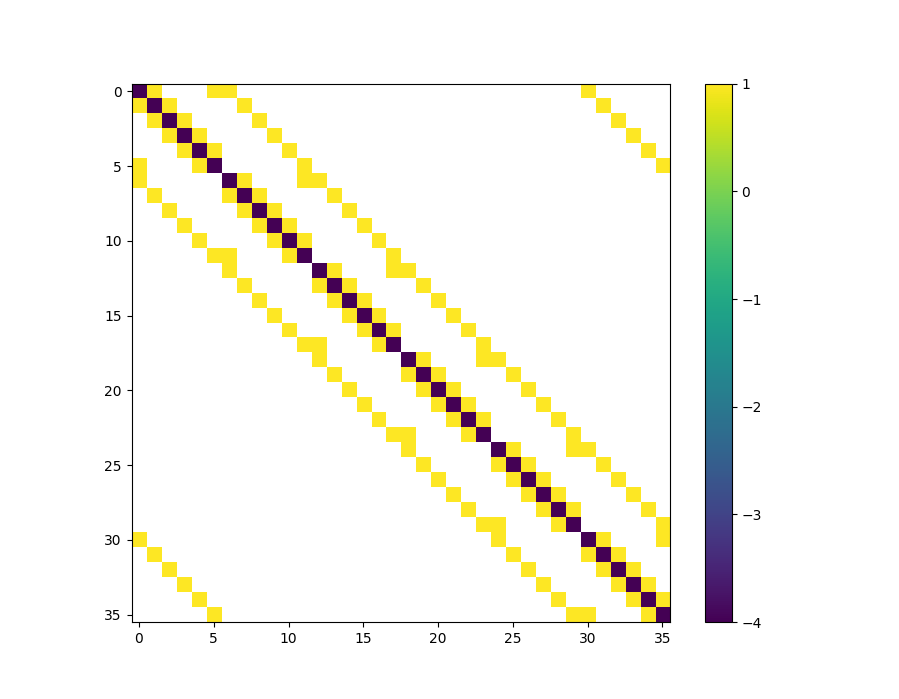
\includegraphics[width=1\textwidth]{plots/2d_laplace_6d1_no_perb.png}
    \caption{2-dimensional discrete laplacian operator with discretization of size \(N_1=N_2=6\) and discretization step size of \(h_1=h_2=1\) for both dimensions show as a heatmap, with zeros removed.}
    \label{fig: 2d laplace heat map}
\end{figure}



% This does not gets us a whole data set of matrices, as mentioned for each matrix entries will have some level of perturbation applied to it.
Because we want sets of distinct matrices, as we need a unique set of matrices for the training and a set for the evaluation of the learned preconditioners. Each nonzero value in the matrices will have some random perturbation applied to it. The simplest way to implement this to perturb the smaller matrices before doing the Kronecker products in equation \ref{eq: 2d laplace Kronecker}. Because the discretization is the same for both dimensions there is only needed to create three unique matrices to get unique entries for the 2-dimensional laplace operator, see equation \eqref{eq: 2d laplace Kronecker perb}. To get small perturbation we use the normal distribution with a mean of 1 and small standard deviation. Note that because the perturbations are done to the smaller matrices and the Kronecker product, the final perturbations will have a distribution of \(N(1,\sigma^2)\cdot N(1,\sigma^2)\). An example of a perturbed matrix can be seen in figure \ref{fig: 2d laplace perp heat map} with an initial perturbation of \(N(1,0.3^2)\).
\begin{equation}\label{eq: 2d laplace Kronecker perb}
    \Delta_{p}\otimes I_{p_1}+ I_{p_2} \otimes \Delta_{p}.
\end{equation}

\begin{figure}[H]
    \center
    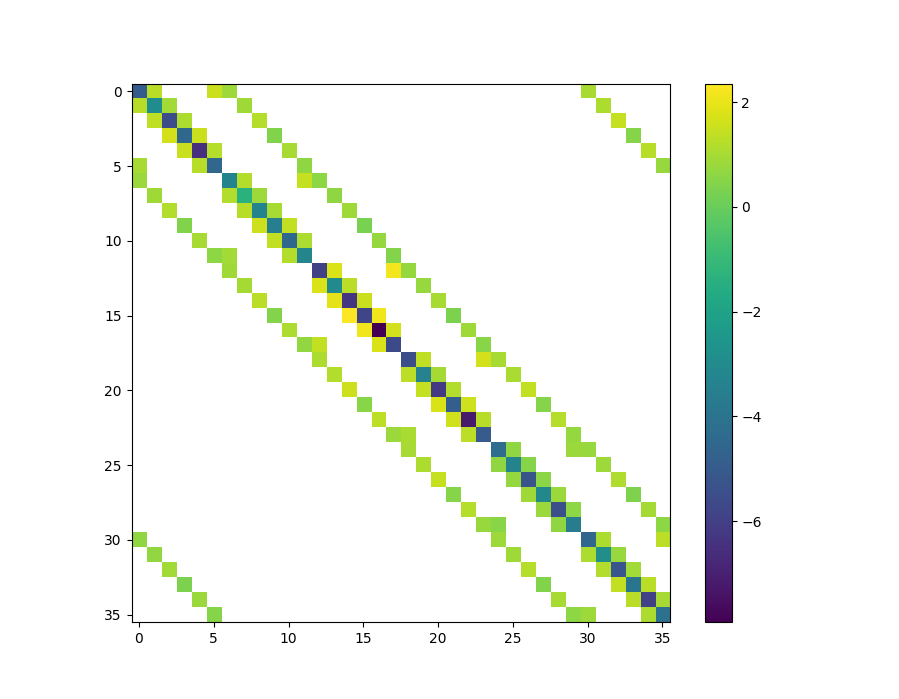
\includegraphics[width=1\textwidth]{plots/2d_laplace_6d1_perp_n_1_0.3.png}
    \caption{2-dimensional discrete laplacian operator with discretization of size \(N_1=N_2=6\) and discretization step size of \(h_1=h_2=1\) for both dimensions with an initial perturbations of \(N(1,0.3^2)\) show as a heatmap, with zeros removed.}
    \label{fig: 2d laplace perp heat map}
\end{figure}

Now that we can generate matrices, we need to determine the parameters of the data generation. These parameters are the discretization size of the 1-dimensional laplace operators and the variance of the initial perturbations. What we would like to have for the solver iteration count is that it is larger than the system size, because then the preconditioner has something to work with. On the other hand we don't want the systems to be too ill-conditioned compared to the size of the system, as we do not want breakdowns to occur for the unpreconditioned linear system, or breakdowns in the exploration of the preconditioner. Therefore we will test four different configurations with 250 matrices each set. The configurations can be seen in table \ref{table: laplace perp param and stat}

\begin{figure}[H]
    \center
    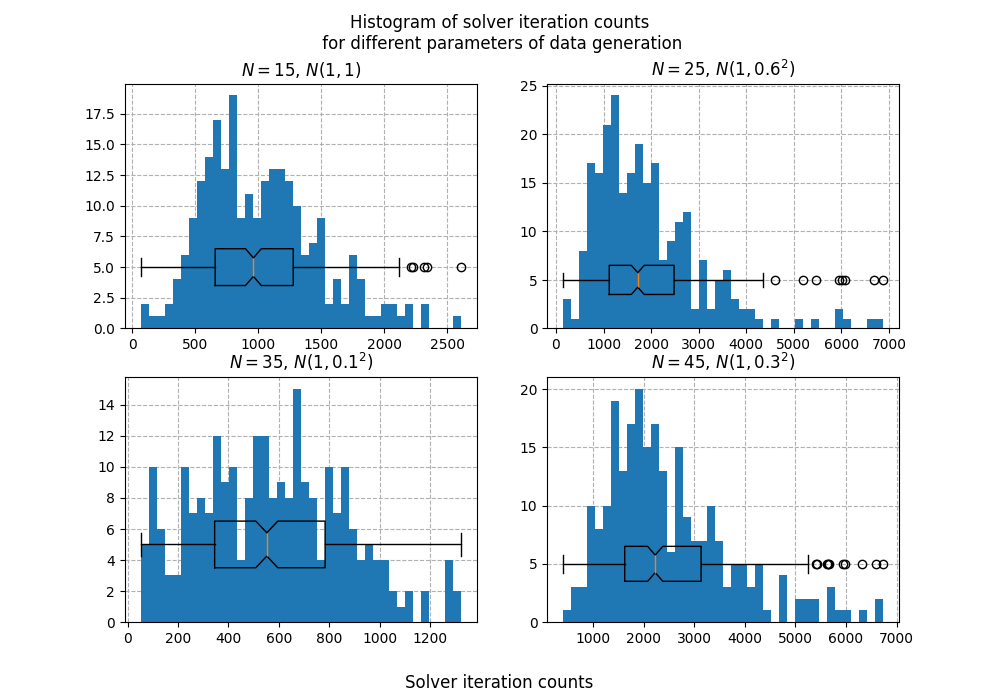
\includegraphics[width=1\textwidth]{plots/laplace_perp_hist.png}
    \caption{Histograms and boxplot of the solver iteration counts for 4 different configurations of the 2-dimensional discrete laplace operator with perturbations, with breakdown occurrences removed.}
    \label{fig: 2d laplace perp hist}
\end{figure}

\begin{table}[H]
    \center
    \begin{tabular}{|l|r|l||r|r|r|r|}
        \hline
        N &\begin{tabular}{@{}l@{}}System \\ Size\end{tabular} & Perturbation & Mean & Median & STD &\begin{tabular}{@{}l@{}}Break \\ downs\end{tabular}\\\hline
        15 &225& \(N(1,1)\) & 1019.1 & 955.5 & 461.11 & 17\\
        25 &625& \(N(1,0.6^2)\) & 1927.6 & 1713 & 1135.8 & 2\\
        35 &1225& \(N(1,0.1^2)\) & 567.2 & 550 & 290.8 & 0\\ 
        45 &2025& \(N(1,0.3^2)\) & 2487.3 & 2218 & 1222.4 & 0\\\hline
    \end{tabular}
    \caption{Parameter configuration and statistic of the four test runs of the 2-dimensional discrete laplace operator with columns corresponding in order to the size of the 1-dimensional discrete laplace operator; the size of the 2-dimensional discrete laplace operator; the initial perturbation distribution; the mean, median, and standard derivation of the solver iterations; the number of systems where a breakdown occurred.}
    \label{table: laplace perp param and stat}
\end{table}

Histograms of the solver iteration count can be seen in figure \ref{fig: 2d laplace perp hist}, and statistic can be seen in table \ref{table: laplace perp param and stat}. The first thing to notice from these four tests is the effect of the perturbations variance has on the solver iteration count. It has a clear positive corelation, meaning with larger variance, the solve iteration count is increased, to the point of becoming too ill-conditioned compared to the system size. This can be seen for configuration with \(N=15\) and perturbation distribution of \(N(1,1)\). What can not be seen in the histograms, because system that had a breakdown occur are removed for readability of the histogram, is that the breakdown that occurred at the latest happened at solver iteration 67337. This is a problem both because that data point is useless for the analysis of the a potential preconditioner, but also because the solving of each of the systems is done in parallel meaning if one of the system take 6 times as long to solve, each learned step has to wait on the that system to breakdown or be solved before it can continues with the learning. Then if the perturbations are smaller, as is the case for the configuration \(N=35\) and \(N(1,0.1^2)\), the solver iteration count are also smaller compared to the size of the system, to the point that a potential preconditioner has very few solver iteration count to improve on. For these reason we will go forward with with the last of the configurations with \(N=45\) and \(N(1,0.3^2)\), as the median solver iteration count is larger than the system size, most iteration count are larger than the system size without having any systems with an occurrences of a breakdown.

With the generation of data the procedure for learning and evaluation of the preconditioners needs to be changed. For each of the learning tests two sets of matrices will be generated of equal amount, one set to be used in the learning of the preconditioner and the other for the evaluation of the learned preconditioner. With this we will avoid overfitting the preconditioner, as the learning algorithm did in the two previous sections \ref{sec: initial learn} and \ref{sec: better exploration}. In the learning algorithm we need a function to determine when a changed is made to the preconditioner was an improvement or if the changed made the preconditioner worse, this we call the improvement function. The functions will be defined and tested in the next section \ref{sec: Improve func}. In the evaluation of the learned preconditioner we will look at three different measures to determine if the preconditioner is good. The first two is the mean and median solver iteration count of the preconditioned system, this will compared against mean and median solver iteration count of the linear systems solved without a preconditioner applied. The third measure will count how many individual systems where the preconditioner reduced the solver iteration compared with using no preconditioner.